%%%%%%%%%%%%%%%%%%%%%%%%%%%%%%%%%%%%%%%%%
% Beamer Presentation
% LaTeX Template
% Version 1.0 (10/11/12)
%
% This template has been downloaded from:
% http://www.LaTeXTemplates.com
%
% License:
% CC BY-NC-SA 3.0 (http://creativecommons.org/licenses/by-nc-sa/3.0/)
%
%%%%%%%%%%%%%%%%%%%%%%%%%%%%%%%%%%%%%%%%%

%----------------------------------------------------------------------------------------
%	PACKAGES AND THEMES
%----------------------------------------------------------------------------------------

\documentclass{beamer}

\mode<presentation> {

% The Beamer class comes with a number of default slide themes
% which change the colors and layouts of slides. Below this is a list
% of all the themes, uncomment each in turn to see what they look like.

%\usetheme{default}
%\usetheme{AnnArbor}
%\usetheme{Antibes}
%\usetheme{Bergen}
%\usetheme{Berkeley}
%\usetheme{Berlin}
%\usetheme{Boadilla}
%\usetheme{CambridgeUS}
%\usetheme{Copenhagen}
%\usetheme{Darmstadt}
%\usetheme{Dresden}
%\usetheme{Frankfurt}
%\usetheme{Goettingen}
%\usetheme{Hannover}
%\usetheme{Ilmenau}
%\usetheme{JuanLesPins}
%\usetheme{Luebeck}
\usetheme{Madrid}
%\usetheme{Malmoe}
%\usetheme{Marburg}
%\usetheme{Montpellier}
%\usetheme{PaloAlto}
%\usetheme{Pittsburgh}
%\usetheme{Rochester}
%\usetheme{Singapore}
%\usetheme{Szeged}
%\usetheme{Warsaw}

% As well as themes, the Beamer class has a number of color themes
% for any slide theme. Uncomment each of these in turn to see how it
% changes the colors of your current slide theme.

%\usecolortheme{albatross}
%\usecolortheme{beaver}
%\usecolortheme{beetle}
%\usecolortheme{crane}
%\usecolortheme{dolphin}
%\usecolortheme{dove}
%\usecolortheme{fly}
%\usecolortheme{lily}
%\usecolortheme{orchid}
%\usecolortheme{rose}
%\usecolortheme{seagull}
%\usecolortheme{seahorse}
%\usecolortheme{whale}
%\usecolortheme{wolverine}

%\setbeamertemplate{footline} % To remove the footer line in all slides uncomment this line
%\setbeamertemplate{footline}[page number] % To replace the footer line in all slides with a simple slide count uncomment this line

%\setbeamertemplate{navigation symbols}{} % To remove the navigation symbols from the bottom of all slides uncomment this line
}

\usepackage{graphicx} % Allows including images
\usepackage{booktabs} % Allows the use of \toprule, \midrule and \bottomrule in tables
\usepackage{amsmath}

%----------------------------------------------------------------------------------------
%	TITLE PAGE
%----------------------------------------------------------------------------------------

\title[Linear Regression]{Multiple Linear Regression} % The short title appears at the bottom of every slide, the full title is only on the title page

\author{David Bethge \& Fabio Ferreira} % Your name
\institute[] % Your institution as it will appear on the bottom of every slide, may be shorthand to save space
{
DHBW Karlsruhe \\ % Your institution for the title page
\medskip
\textit{} % Your email address
}
\date{\today} % Date, can be changed to a custom date

\begin{document}

\begin{frame}
\titlepage % Print the title page as the first slide
\end{frame}

\begin{frame}
\frametitle{Recommended Literature}

\begin{figure}
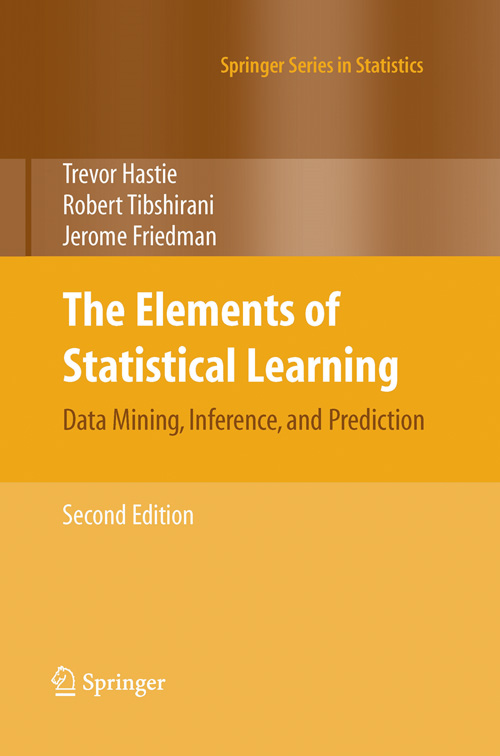
\includegraphics[width=0.4\linewidth]{figures/03/Literature.jpg}
\end{figure}


\end{frame}
\begin{frame}
\frametitle{Overview} % Table of contents slide, comment this block out to remove it
\tableofcontents % Throughout your presentation, if you choose to use \section{} and \subsection{} commands, these will automatically be printed on this slide as an overview of your presentation
\end{frame}


%----------------------------------------------------------------------------------------
%	PRESENTATION SLIDES
%----------------------------------------------------------------------------------------

%------------------------------------------------
\section{basics} % Sections can be created in order to organize your presentation into discrete blocks, all sections and subsections are automatically printed in the table of contents as an overview of the talk
%------------------------------------------------

\subsection{vector and matrix algebra} % A subsection can be created just before a set of slides with a common theme to further break down your presentation into chunks

\begin{frame}
\frametitle{vector}
We begin by defining a vector, a set of n numbers which we shall write in the form
$$
\vec{a} = 
\begin{pmatrix}
a_{1}\\
a_{2} \\
...\\
a_{n}
\end{pmatrix}
$$
is called a column vector of the size ($n \times 1$).
\newline
If n numbers are arranged in a horizontal array, as in
$$
\vec{a} = 
\begin{pmatrix}
a_{1} &
a_{2} &
... &
a_{n}
\end{pmatrix}
$$
then $\vec{a}$ is called a row vector of the size ($1 \times n$).

\end{frame}

\begin{frame}
\frametitle{matrix}
An $n \times p$ matrix A has n columns and p rows: 
$$
A = 
\begin{pmatrix} 
a_{11} & ... & a_{1p} \\
... & \ddots &...\\
a_{n1} & ... & a_{np} & 
\end{pmatrix}
$$
We will write $a_{ij}$ for the element in column i and row j.
\newline
We will assume $a_{ij} \in \mathbb{R}$. 
\newline
\newline
Most of the datasets we use in machine learning will have the form of the denoted matrix A with n observations and p variables.


\end{frame}


\begin{frame}
\frametitle{mathematical operations on vectors and matrices}

\begin{itemize}
\item scalar multiplication
\item matrix multiplication
\item sum of matrices
\item tensor matrices
\item inverse matrices
\end{itemize}

\end{frame}



\subsection{expectation value, variance}

\begin{frame}
\frametitle{expectation value}
In probability theory, the expected value of a random variable, intuitively, is the long-run average value of repetitions of the experiment it represents. 
\newline
For example, the expected value in rolling a six-sided dice is 3.5.
\newline
$$
\mathbb{E}[X] = \int_{-\infty}^{\infty} \! x f(x) \, \mathrm{d}x
$$

Assume $$X= 
\begin{pmatrix}
X_{1} & X_{2} & ... & X_{p}
\end{pmatrix}
$$
is a p-dimensional random vector. 
\newline 
Then its expectation value vector is:
$$
\mathbb{E}[X] =
\begin{pmatrix}
\mathbb{E}[X_{1}] \\
\mathbb{E}[X_{2}]\\
... \\
\mathbb{E}[X_{p}]
\end{pmatrix}
$$
\end{frame}



\begin{frame}
\frametitle{mean vector}
Often the distribution of X is unknown so expectation value cannot be calculated. To estimate the expectation value we will use the (empirical) mean vector.
\newline
The mean of a sample of size n is defined as:
$$
\bar{X} = \frac{1}{n} (X_1 +X_2 + ...+X_n) =  \frac{1}{n} \sum_{i = 1}^{n}X_i
$$
\newline 
As with $\mathbb{E}[X], \bar{X}$ can be also written as a vector: 
$$
\bar{X} =
\begin{pmatrix}
\bar{X}_{1} \\
\bar{X}_{2}\\
... \\
\bar{X}_{p}
\end{pmatrix}
= 
\begin{pmatrix}
 \frac{1}{n} \sum_{i = 1}^{n}X_{1i} \\
 \frac{1}{n} \sum_{i = 1}^{n}X_{2i} \\
... \\
 \frac{1}{n} \sum_{i = 1}^{n}X_{pi} 
\end{pmatrix}
$$
Here we calculate the mean value of each variable by summing over the observations (and dividing by the number of observations).



\end{frame}

\begin{frame}
\frametitle{variance}

In probability theory and statistics, variance is the expectation of the squared deviation of a random variable from its mean. Informally, it measures how far a set of (random) numbers are spread out from their average value.


\begin{align*}
Var(X) &= \mathbb{E}[(X - \mathbb{E}[X])^2] \\
&= E[X^2 - 2XE[X] + E[X]^2] \\
&= E[X^2] - 2E[X]E[X] + E[X]^2 \\
&= E[X^2] - E[X]^2
\end{align*}


\end{frame}

\section{notation}



\begin{frame}
\frametitle{dataset notation}
\begin{itemize}
\item $i$: index of the observation or observation
\item $j$: index of a variable/feature
\item $x_{ij}$: value of the j-th variable for the i-th observation,
where $i = 1, 2, . . ., n$ and $j = 1, 2, . . . , p$.
\item $X$: a $n\times p$ matrix whose (i, j)-th element is x $ij$
\item $x^j$: column vector of X
\item $x_{i}$: row vector of X
\end{itemize}
$$
X = 
\begin{pmatrix} 
x_{11} & ...& x_{1j} & ... & x_{1p} \\
... & ... &...& ...& ...\\
x_{i1} & ... & x_{ij} & ... &x_{ip}\\
... & ...& ...& ...& ...\\
x_{n1} & ... & x_{nj}& ...& x_{np} & 
\end{pmatrix}
$$

\end{frame}


\begin{frame}
\frametitle{example for dataset notation}
\begin{itemize}
\item n: number of distinct data points, or observations, in the sample
\item p: number of variables that are available for prediction
\end{itemize}
\bigskip
Example: Wage data set consists of 12 variables for 3,000 people
\begin{itemize}
\item n = 3,000 observations
\item p = 12 variables (such as year, age, wage, and more).
\end{itemize}

\end{frame}




%------------------------------------------------

\section{simple linear regression}
\begin{frame}
\Huge{linear regression}
\newline
\newline
\normalsize
\textit{ "Essentially, all models are wrong, but some are useful" } (George Box)
\end{frame}

\subsection{introduction}
\begin{frame}
\frametitle{introduction}
Now as we introduced the very basics of linear algebra needed for machine learning, we have a quick look at the very popular linear regression method.
\newline
\textbf{Basic idea}:
\newline
Use data to identify linear relationships among variables and use these relationships to make predictions.
\begin{figure}
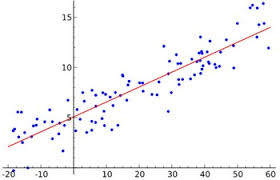
\includegraphics[width=0.45\linewidth]{figures/03/linear_regression.jpg}
\end{figure}
%link: https://upload.wikimedia.org/wikipedia/commons/thumb/3/3a/Linear_regression.svg/2000px-Linear_regression.svg.png
\end{frame}


\begin{frame}
\frametitle{motivation}
We look at a model with the following parameters:
\begin{itemize}
\item unknown parameters $\beta$
\item independent variables $X$
\item dependent variable $y$
\end{itemize}
and want to estimate a function $f(X,\beta)$, with:
\begin{equation}
y \approx f(X,\beta)
\end{equation}



\end{frame}

\begin{frame}
\frametitle{model}
To further specify the function $f(...)$  \textbf{ we restrict ourselves to a linear relationship}:
\begin{block}{Model assumption}
$y = \beta_0 + \beta_1 x_1 + \beta_2 x_2 + ... + \beta_p  x_p  + \epsilon= \beta_0 + \sum_{i = 1}^p \beta_i x_i + \epsilon$
\end{block}

But in practice the linear assumption does not always hold.
\newline
Nonetheless linear regression has proven to be a important tool in practice.
\end{frame}

\begin{frame}
\frametitle{simple linear model}
We can observe $n$ data points $(x_1,y_1),(x_2, y_2), ..., (x_n, y_n)$, then we can write for each observation $i$: 
\begin{equation*}
y_i = \beta_0 + \beta_1 x_i + \epsilon_i
\end{equation*}
with 
\begin{equation*}
\epsilon \sim N(0,\sigma^2)
\end{equation*}
\begin{itemize}
\item Here, the noise $\epsilon_i$ represents the fact that our data won’t fit the model perfectly (we model it gaussian).
\item Note that the intercept $\beta_0$, the slope $\beta_1$, and the noise
variance $\sigma^2$
are all treated as fixed (i.e., deterministic) but unknown quantities
\end{itemize}
\end{frame}

\begin{frame}
\frametitle{estimating the simple linear model}
Since we observe: $(x_1,y_1),(x_2, y_2), ..., (x_n, y_n)$, we need to solve the following optimization problem:
\begin{equation*}
\min_{\beta_0, \beta_1} \sum_{i = 1}^n [y_i- (\beta_0 + \beta_1 x_i)]^2 = \sum_{i = 1}^n [y_i- \hat{y_i}]^2  = \sum_{i = 1}^n e_i^2
\end{equation*}
\begin{itemize}
\item $\hat{y_i}$ is called the prediction for observation $i$
\item $e_i = y_i  - \hat{y_i}$ is the i'th residual
\end{itemize}
Solution:
\begin{equation*}
\hat{\beta_1} = \frac{\sum_{i = 1}^n x_i y_i - \frac{1}{n} \sum_{i = 1}^{n}\sum_{i = 1}^n x_i y_i }{\sum_{i = 1}^n x_i^2 -\frac{1}{n} (\sum_{i = 1}^n x_i )^2 } = r \frac{s_y}{s_x}
\end{equation*}
\begin{equation*}
\hat{\beta_0} = \bar{y} - \hat{\beta_1} \bar{x}
\end{equation*}
\end{frame}


\begin{frame}
\frametitle{visualization of the simple linear model}
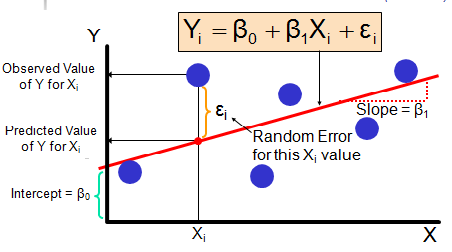
\includegraphics[width=0.9\textwidth]{figures/03/regressioncurv.png}
\newline
\tiny("https://madhureshkumar.files.wordpress.com/2015/07/regressioncurv.png")
\end{frame}

\subsection{statistical properties}

\begin{frame}
\frametitle{accuracy of the coefficient estimates}
The standard error of an estimator reflects how it varies
under repeated sampling.
\begin{equation*}
SE(\hat{\beta_1})^2 = \frac{\sigma^2}{\sum_{i = 1}^n (x_i - \bar{x})^2}
\end{equation*}
\begin{equation*}
SE(\hat{\beta_0})^2 =\sigma^2 [\frac{1}{n} +\frac{\bar{x}^2}{\sum_{i = 1}^n (x_i - \bar{x})^2}]
\end{equation*}
with $\sigma^2 = Var(\epsilon)$
\newline
We can also show that our estimate satisfies:
\begin{equation*}
\hat{ \beta_i } \sim N(\beta_i,  \frac{\sigma^2}{\sum_{i = 1}^n (x_i - \bar{x})^2})
\end{equation*}

Now with the standard errors we can calculate confidence intervals: A 95\% confidence interval ($\alpha = 0.05$) is defined as a range of
values such that with 95\% probability, the range will
contain the true unknown value of the parameter:
\begin{equation*}
\beta_1 \pm t_{n-p}^{1-\alpha/2} \sqrt[]{SE(\hat{\beta_1}^2) }
\end{equation*}
\end{frame}


\begin{frame}
\frametitle{accuracy of the coefficient estimates (2)}
That is, there is approximately a 95\% chance that the interval
\begin{equation*}
[\beta_1 - t_{n-p}^{1-\alpha/2}\sqrt[]{SE(\hat{\beta_1})^2}, \beta_1 + t_{n-p}^{1-\alpha/2} \sqrt[]{SE(\hat{\beta_1})^2} ]
\end{equation*}
will contain the true value of $\beta_1$ (under a scenario where we got
repeated samples like the present sample)
\end{frame}

\begin{frame}
\frametitle{hypothesis testing}
Standard errors can also be used to perform hypothesis
tests on the coefficients. The most common hypothesis test
involves testing the null hypothesis of:
\begin{itemize}
\item $H_o$: There is no relationship between X and Y
versus the alternative hypothesis
\item $H_1$: There is some relationship between X and Y .
\end{itemize}

Mathematically, this corresponds to testing:
\begin{itemize}
\item $H_o$: $\beta_1 = 0$
\item $H_1$: $\beta_1 \neq 0 $
\end{itemize}
since if $\beta_1 = 0$ then the model reduces to $y = \beta_0 + \epsilon$, and
X is not associated with Y .
\end{frame}

\begin{frame}
\frametitle{hypothesis testing}
To test the null hypothesis, we compute a t-statistic, given
by:
\begin{equation*}
t = \frac{ \hat{\beta_1} - 0 }{SE(\hat{\beta_1})}
\end{equation*}
This will have a t-distribution with $n-2$ degrees of
freedom, assuming $\beta_1 = 0$.
\newline
Using statistical software, it is easy to compute the
probability of observing any value equal to $\mid t \mid$ or larger. We
call this probability the p-value.
\end{frame}


\subsection{model evaluation}
\begin{frame}
\frametitle{assessing the overall accuracy of the model}

\begin{itemize}
\item We compute the Residual Standard Error:
\begin{equation*}
RSE = \sqrt[]{\frac{1}{n-2} RSS} = \sqrt[]{\frac{1}{n-2} \sum_{i=1}^n (y_i -\hat{y_i})^2}
\end{equation*}
\item R-squared or fraction of variance explained is:
\begin{equation*}
R^2  = \frac{TSS - RSS}{TSS} = 1- \frac{RSS}{TSS}
\end{equation*}
where $TSS$ is the total sum of squares: $\sum_{i=1}^n (y_i -\bar{y})^2$
\item R-squared is always $\in [0,1]$, whereby 1 represents a perfect fit 

\item decomposition of the variance: 
\begin{equation*}
\underbrace{\sum_{i = 1}^n (y_i-\bar{y})^2}_\text{TSS} = \underbrace{\sum_{i = 1}^n \hat{e_i}^2}_\text{RSS} + \underbrace{\sum_{i = 1}^n (\hat{y_i}-\bar{y})^2}_\text{ESS} 
\end{equation*}
\end{itemize}

\end{frame}

\begin{frame}
\frametitle{R-squared}
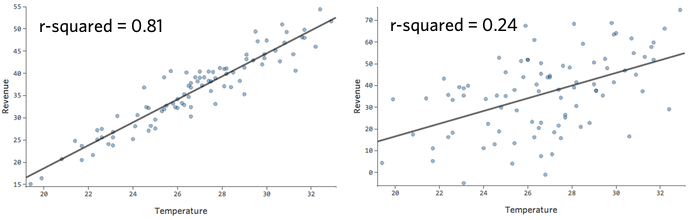
\includegraphics[width = 0.9\textwidth]{figures/03/Good-and-bad-fits2.png}
\newline
be careful using R-squared as the only measure for quality of the model
\begin{itemize}
\item R-squared increases inherently with the number of predictors, even if the added variables are not explaining something
\item use the adjusted $R^2_{adj.}$ instead: $1-(1-R^2)\frac{n-1}{n-p-1}$
\end{itemize}
\end{frame}

\begin{frame}
\frametitle{linear regression is intriguing}
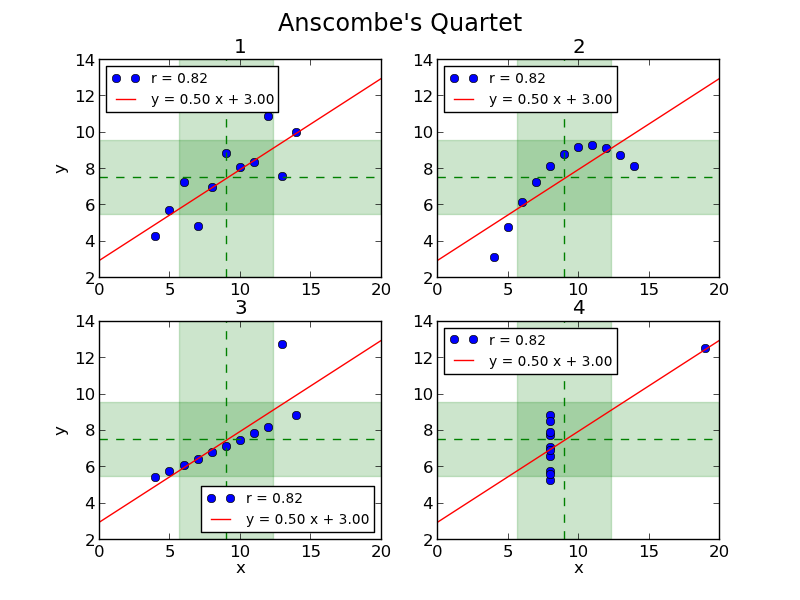
\includegraphics[width = 0.9\textwidth]{figures/03/anscombe.png}
\newline
%"http://informatique-python.readthedocs.io/fr/latest/_images/anscombe.png"
\end{frame}


\subsection{prediction}

\begin{frame}
\frametitle{prediction}
If the $\beta$ parameters are estimated on the training data, now we can make predictions on new (unseen) data. From now on we call the estimated parameters $\hat{\beta}$ and a new unseen data points $X_{0}$. So the prediction for the given $y$ is:
\begin{equation*}
\hat{y} = \hat{\beta_o} + X_{0} \hat{\beta_1}
\end{equation*}
Example: We want to find out how the number of customers affects the sales of a supermarket ($\#$sales $\approx$ $\#$customers). 
\newline
So let's say we found out that $(\hat{\beta_0} , \hat{\beta_1})$ = $(-2, 0.4)$, which is a very considerate estimate. So if we see $20$ customers coming in the supermarket: the estimate sale would be: $\hat{y} = -2+ 0.4*20 = 6$.
\end{frame}


\section{multiple linear regression}
\begin{frame}
\Huge{multiple linear regression}
\newline
\newline
\normalsize
\textit{ Beyond dimension 2 }
\end{frame}


\begin{frame}
\frametitle{notation}
In the multivariate case we want to use more than one variable (it is also called multiple regression):
\begin{block}{Linear model form}
$y = \beta_0 + \beta_1 x_1 + \beta_2 x_2 + ... + \beta_p  x_p  + \epsilon= \beta_0 + \sum_{i = 1}^p \beta_i x_i + \epsilon$
\end{block}
Can be written as:
\begin{block}{Matrix notation}
$y =  X  \beta + e$
\end{block}

\end{frame}


\begin{frame}
\frametitle{example}
Let's recall our matrix notation:
\begin{table}[]
\centering
%\caption{My caption}
\label{my-label}
\begin{tabular}{|l|lll}
\hline
          & \multicolumn{1}{l|}{\begin{tabular}[c]{@{}l@{}}Coffein \\ Consumption ($x_1$)\end{tabular}} & \multicolumn{1}{l|}{\begin{tabular}[c]{@{}l@{}}noise\\  level ($x_2$)\end{tabular}} & \multicolumn{1}{l|}{\begin{tabular}[c]{@{}l@{}}power of \\ concentration ($y$)\end{tabular}} \\ \hline
student 1 & 3                                                                                          & 0                                                                                  & 85                                                                                         \\ \cline{1-1}
student 2 & 0                                                                                          & 6                                                                                  & 41                                                                                         \\ \cline{1-1}
student 3 & 1                                                                                          & 3                                                                                  & 60                                                                                         \\ \cline{1-1}
student 4 & 4                                                                                          & 9                                                                                  & 53                                                                                         \\ \cline{1-1}
...       & ...                                                                                        & ...                                                                                & ...                                                                                        \\ \cline{1-1}
\end{tabular}
\end{table}
\end{frame}


\begin{frame}
\frametitle{variable assignment}
This is how we initialize our matrices for the multiple regression:
\bigskip
\bigskip
$
X = 
\begin{bmatrix} 
1 & x_{11} & ...& x_{1j} & ... & x_{1p} \\
...& ... & ... &...& ...& ...\\
1 & x_{i1} & ... & x_{ij} & ... &x_{ip}\\
... & ...& ...& ...& ...\\
1 & x_{n1} & ... & x_{nj}& ...& x_{np} & 
\end{bmatrix}
$
\quad
 $
 y = 
 \begin{bmatrix}
y_1 \\
y_2 \\
... \\
y_n 
\end{bmatrix}
$ 
 $
 e = 
 \begin{bmatrix}
e_1 \\
e_2 \\
... \\
e_n 
\end{bmatrix}
$  
 $
 \beta = 
 \begin{bmatrix}
\beta_0 \\
\beta_1 \\
... \\
\beta_p 
\end{bmatrix}
$  

\textbf{Question}: Why is there a column of ones in X?
\end{frame}

\begin{frame}
\frametitle{Assumptions}
Regressor matrix:
\begin{itemize}
\item X is stochastic
\item X has full rank: $Rank(X) = p$
\end{itemize}
\bigskip
Error Term:
$e|X \sim (0, \sigma^2 I_n)$
\begin{itemize}
\item strict exogeneity: $\mathbb{E}[e_i|X] = 0 \quad \forall i$ 
\item conditioned homoskedacity: $Var[e_i|X] = \sigma^2 \quad  i\neq j$
\item conditionially uncorrelated:  $\mathbb{E}[e_ie_j|X] = 0 \quad \forall i$ 
\item sometimes we assume: $e|X \sim N(0, \sigma^2 I_n)$
\end{itemize}
\end{frame}


\begin{frame}
\frametitle{OLS estimation}
Goal: minimize the distances between true and predicted values (ordinary least squares)
\begin{align*} 
min_{\beta} &= \frac{\partial }{\partial \beta} (y - X\beta)'(y - X\beta) = \frac{\partial }{\partial \beta} \hat{e}'\hat{e} \\
    &= \frac{\partial }{\partial \beta} ( y'y -2\beta'X'y + \beta'X'X\beta ) \\
  &= -2X'y   +2 X'Xb \\
  X'y &= X'Xb
\end{align*}

optimizing $\beta$ yields the regression coefficient to be:
\begin{block}{Coefficient estimator}
$ b = (X'X)^{-1}X'y $
\end{block}


\end{frame}


\begin{frame}
\frametitle{geometrical understanding}

\begin{figure}
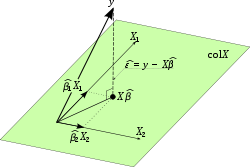
\includegraphics[width=0.7\linewidth]{figures/03/geometry.png}
\end{figure}
%link: https://upload.wikimedia.org/wikipedia/commons/thumb/8/87/OLS_geometric_interpretation.svg/250px-OLS_geometric_interpretation.svg.png
\end{frame}

\begin{frame}
\frametitle{properties of the OLS estimator b}
It is (under some specific assumptions) the best linear unbiased estimator (BLUE):
\newline
b is unbiased:
\begin{equation*}
\mathbb{E}[b] = \mathbb{E}[(X'X)^{-1}X'y] = \mathbb{E}[(X'X)^{-1}X'(X\beta +e)] = (X'X)^{-1}X'X\beta = \beta
\end{equation*}


\begin{align*} 
Var[b] =& Var[(X'X)^{-1}X'y]\\
=& Var[\beta + (X'X)^{-1}X'e]\\
=&Var[(X'X)^{-1}X'e] \\
=& (X'X)^{-1}X' Var[e] X (X'X)^{-1} \\
=&  \sigma^2(X'X)^{-1}
\end{align*}

We can also write (normality not always given):
\begin{block}{properties of the OLS estimate}
$ b \sim N(\beta , \sigma^2(X'X)^{-1} ) $
\end{block}

\end{frame}

\begin{frame}
\frametitle{prediction}
Now we want to do a prediction for a given data matrix $X_0$. First we estimate b and then we can infer the predicted values $\hat{y}$:
\begin{align*} 
\hat{y} =& X_0 b \\
=& X_0 (X'X)^{-1}X'y \\
\end{align*}
We can show that the prediction is unbiased:
\begin{align*} 
\mathbb{E}[\hat{y}] = & \mathbb{E}[X_0 b] \\
=&\mathbb{E}[ X_0 (X'X)^{-1}X'y ]\\
=& X_0 (X'X)^{-1}X' \mathbb{E}[ X\beta +e ]\\
=& X_0 (X'X)^{-1}X'X\beta +  X_0 (X'X)^{-1}X'X\mathbb{E}[e ]\\
=& X_0 (X'X)^{-1}X'X\beta = X_0 \beta \\
\end{align*}
\end{frame}


\begin{frame}
\frametitle{prediction interval (1)}
We learned how to calculate a point estimate for y, but it is often far more useful to get an prediction interval: 
\begin{equation*}
[\hat{y_0} - t_{n-p}^{1-\alpha/2} \sqrt[]{\hat{Var}_{pred}(X_0)}, \hat{y_0} + t_{n-p}^{1-\alpha/2} \sqrt[]{\hat{Var}_{pred}(X_0)}  ]
\end{equation*}
and 
\begin{equation*}
\hat{Var}_{pred}(X_0)  =  \sigma^2 (I_0 + X_0(X'X)^{-1} X_0'
\end{equation*}

\end{frame}
 \begin{frame}
 \frametitle{prediction interval (2)}
 \begin{figure}
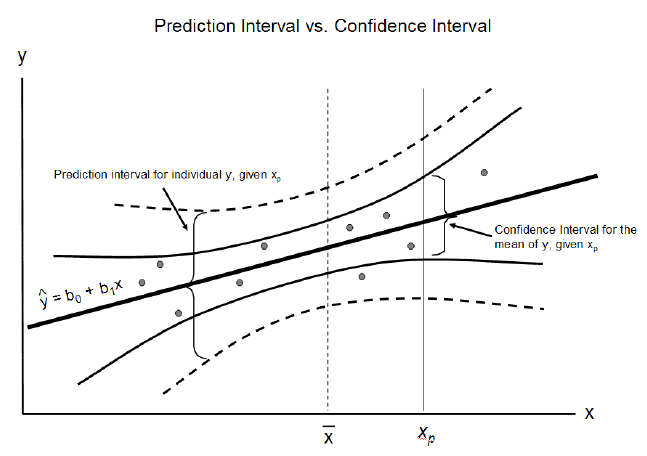
\includegraphics[width=0.8\linewidth]{figures/03/Prediction-Interval-vs-Confidence-Interval.png}
%link: https://www.researchgate.net/profile/Eugene_Wang/publication/267958281/figure/fig1/AS:295290067275778@1447414046375/Prediction-Interval-vs-Confidence-Interval.png
\end{figure}
 \end{frame}


\subsection{Assessing goodness of fit}
\begin{frame}
\frametitle{$R^2$}
In statistics, the coefficient of determination, denoted $R^2$, is the proportion of the variance in the dependent variable that is predictable from the independent variable(s):

\begin{equation}
R^2 = \frac{ESS}{TSS} = 1- \frac{RSS}{TSS} = 1- \frac{(y-\hat{y})'(y-\hat{y})}{\sum_{i = 1}^{n}{ (y_i - \bar{y} )^2}}= 1- \frac{\hat{e}'\hat{e}}{y'y - n\bar{y}^2}
\end{equation}
Ideally $R^2$ is close to $1$, since then the predicted value $\hat{y}$ and the true values $y$ are very close (residuals $\hat{e}'\hat{e} \rightarrow 0$). 
\end{frame}

\begin{frame}
\frametitle{adjusted $R^2$ }
Unfortunately $R^2$ has some shortcomings, that are corrected with an adjusted $R^2$
\begin{itemize}
\item R2 increases with every predictor added to a model. As R2 always increases and never decreases, it can appear to be a better fit with the more terms you add to the model (misleading).
\item Similarly, if your model has too many terms and too many high-order polynomials you can run into the problem of over-fitting the data.
\end{itemize}
Adjusted R2 also indicates how well terms fit a curve or line, but adjusts for the number of terms in a model. If you add more and more useless variables to a model, adjusted r-squared will decrease. If you add more useful variables, adjusted r-squared will increase.

\begin{equation}
R^2_{adj.} = 1- (1-R^2) \frac{n-1}{n-p-1}
\end{equation}
\end{frame}

\begin{frame}
\frametitle{the effect of outliers}
\begin{figure}
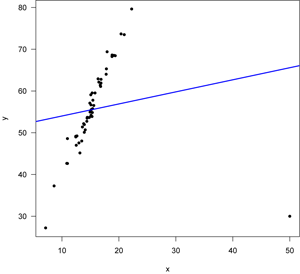
\includegraphics[width=0.8\linewidth]{figures/03/outlier.png}
%link: http://strata.uga.edu/8370/rtips/images/outlier.png
\end{figure}
\end{frame}



\begin{frame}
\frametitle{pros \& cons of multiple linear regression}
\begin{itemize}
\item easy and intuitive "simple" approach
\item it works in many cases: even when it doesn’t fit the data exactly, we can use it to find the nature of the relationship between the two variables
\item It assumes there is a linear relationship between the variables which is incorrect sometimes
\item it is very sensitive to the anomalies in the data (or outliers)
\item it is prone to overfitting of the data (i.e some noisy data also considered as useful data)
\end{itemize}

\end{frame}



\section{algorithms}
\section{algorithms}
\begin{frame}
\Huge{Algorithms:
\newline
Ridge Regression, LASSO, Nearest Neighbor}
\newline
\newline
\normalsize
\textit{ Digging deeper}
\end{frame}
\subsection{ridge regression}
\begin{frame}
\frametitle{ridge regression - motivation}
\textbf{Motivation: too many predictors}
\begin{itemize}
\item It is not unusual to see the number of input variables greatly exceed the number of observations, e.g. micro-array data analysis, environmental pollution studies.
\item With many predictors, fitting the full model without penalization will result in large prediction intervals, and OLS regression estimator may not uniquely exist.
\end{itemize}
\bigskip
\textbf{Motivation: ill-conditioned $X$}
\begin{itemize}
\item Because the OLS estimates depend upon $(X′X)^{-1}$, we would have problems in computing $b$ if $X′X$ is not invertable.
\end{itemize}
\end{frame}

\begin{frame}
\frametitle{ridge regression - derivation}
One way out of this situation is to shrink the regression coefficients via \textbf{ridge regression}.
\newline
In ridge regression we penalize big values for the coefficient estimator. Thus our optimization problem looks like this:
\begin{align*} 
min_{\beta} &= \sum_{i=1}^n (y_i - \hat{y_i})^2 + \lambda \sum_{j=1}^p (\beta_j^2) \\
&=\frac{\partial }{\partial \beta} (y - X\beta)'(y - X\beta)  + \lambda \beta'\beta \\
    &= \frac{\partial }{\partial \beta} ( y'y -2\beta'X'y + \beta'X'X\beta + \lambda \beta'\beta ) \\
  &= -2X'y   +2 X'X\hat{\beta}_{R}+ 2\lambda\hat{\beta}_{R} \\
  X'y &= \hat{\beta}_{R} (X'X + \lambda I_p)
\end{align*}

\end{frame}

\begin{frame}
\frametitle{ridge regression}
\begin{block}{ridge regression coefficient}
$  \hat{\beta}_{R} = (X'X + \lambda I_p)^{-1}X'y $
\end{block}
Thus via Ridge regression potential instability in the OLS estimator $b =(X'X )^{-1}X'y $ could be improved by adding a small constant value $\lambda$ to the diagonal entries of the matrix $X′X$ before taking its inverse.
\newline
The penalty term is $\lambda$ (a pre-chosen constant) times the squared norm of the $\beta$ vector. This means that if the $\beta_j$'s take on large values, the optimization function is penalized. We would prefer to take smaller $\beta_j$'s, or $\beta_j$'s that are close to zero to drive the penalty term small.
\newline
\newline
\textbf{Question}: Which $\lambda$ value results in the normal OLS regression?
\newline
Hint:
\begin{equation*}
\sum_{i=1}^n (y_i - \hat{y_i})^2 + \lambda \sum_{j=1}^p (\beta_j^2) 
\end{equation*} 
\end{frame}

\begin{frame}
\frametitle{shrinking of coefficient estimates}
\begin{figure}
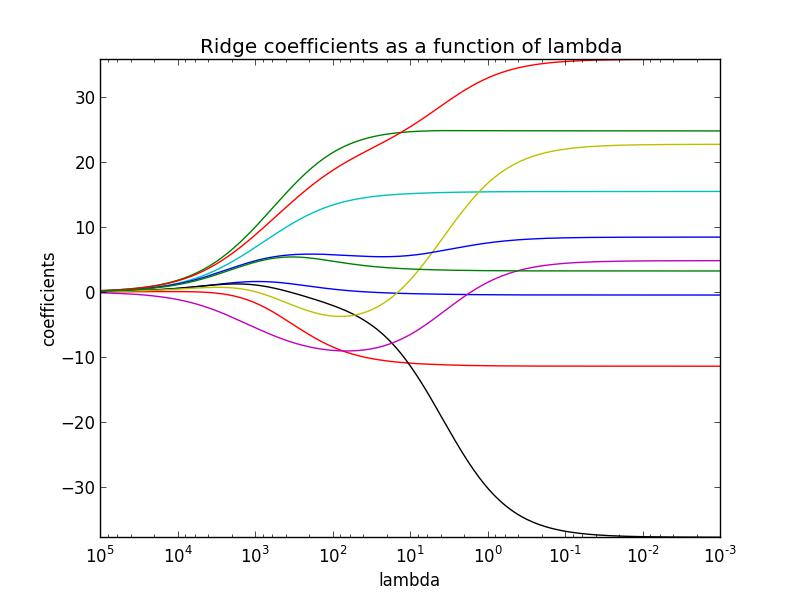
\includegraphics[width=0.8\linewidth]{figures/03/ridge.jpeg}
%link: https://statcatinthehat.files.wordpress.com/2014/07/ridge_s.jpeg
\end{figure}
\end{frame}
\subsection{LASSO}
\begin{frame}
\frametitle{LASSO}
\textbf{LASSO} (least absolute shrinkage and selection operator) is similar to ridge regression. In LASSO our optimization problem looks like this: 
\begin{align*} 
min_{\beta} &= \sum_{i=1}^n (y_i - \hat{y_i})^2 + \lambda \sum_{j=1}^p |\beta_j| \\
\end{align*}



\begin{itemize}
\item LASSO forces certain coefficients to be set to zero effectively choosing a simpler model that does not include those coefficients (better interpretability).
\item This idea is similar to ridge regression, in which the sum of the squares of the coefficients is forced to be less than a fixed value, though in the case of ridge regression, this only shrinks the size of the coefficients, it does not set any of them to zero.
\end{itemize}

\end{frame}


\begin{frame}
\frametitle{LASSO vs. Ridge}
\begin{figure}
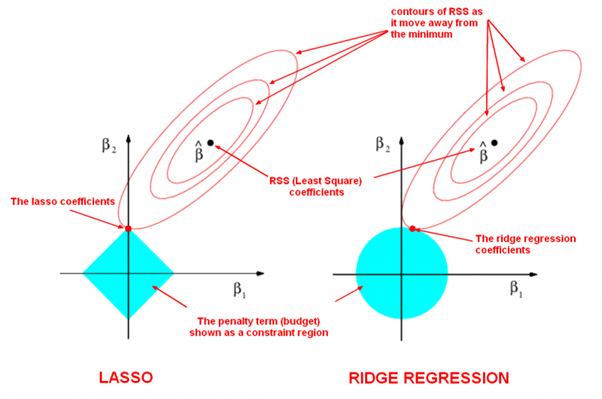
\includegraphics[width=0.9\linewidth]{figures/03/lasso_vs_ridge.png}
%link: https://qph.fs.quoracdn.net/main-qimg-2a88e2acc009fa4de3edeb51e683ca02
\end{figure}
\end{frame}



\subsection{nearest neighbor method}
\begin{frame}
\frametitle{Nearest Neighbor Method}
\Huge{Nearest Neighbor Method}
\newline
\newline
\normalsize
\textit{"Sometimes our neighbors define who we are."}
\end{frame}


\begin{frame}
\frametitle{motivation}
Nearest neighbor search (NNS), as a form of \textbf{proximity} search, is the optimization problem of finding the point in a given set that is closest (or most similar) to a given point. 
\newline
Closeness is typically expressed in terms of a dissimilarity function: the less similar the objects, the larger the function values. 
\newline
The most popular method is the \textbf{k-nearest neighbor method}.
\end{frame}

\begin{frame}
\frametitle{k-nearest neighbor}
identifies the top $k$ nearest neighbors to the query:
\begin{figure}
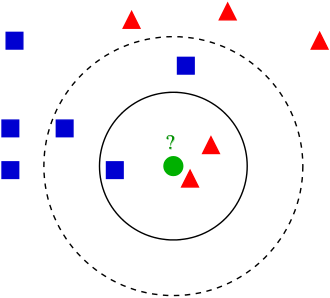
\includegraphics[width=0.4\linewidth]{figures/03/KNN.png}
%link: https://upload.wikimedia.org/wikipedia/commons/thumb/e/e7/KnnClassification.svg/330px-KnnClassification.svg.png
\end{figure}
\tiny
Example of k-NN classification. The test sample (green circle) should be classified either to the first class of blue squares or to the second class of red triangles. If $k = 3$ (solid line circle) it is assigned to the second class because there are 2 triangles and only 1 square inside the inner circle. If k = 5 (dashed line circle) it is assigned to the first class (3 squares vs. 2 triangles inside the outer circle).
\end{frame}
\begin{frame}
\frametitle{k-nearest neighbor algorithm}
Suppose we have pairs ${ (X_{1},Y_{1}),\dots ,(X_{n},Y_{n})}$ and we want to calculate the predicted value for $x_0$
\begin{itemize}
\item calculate the distance between each pair and $x_0$
\item reorder the training data such that: $\|X_{{(1)}}-x_0\|\leq \dots \leq \|X_{{(n)}}-x_0\|$
\item select the first k data points (those with minimal distance)
\item assign $x_0$ the value of the k-nearest ($Y_i$) values:
	\begin{itemize}
	\item \textbf{classification}: assign the label which is most frequent among the $k$ training samples nearest to $x_0$ (majority voting)
    \item \textbf{regression}
    assign the predicted value to be the mean value of its k-neighbors
	\end{itemize}
\end{itemize}
Under some circumstances, it can be advantageous to weight points such that nearby points contribute more to the regression than faraway points
\end{frame}

\begin{frame}
\frametitle{k-nearest neighbors}
\begin{figure}


\begin{minipage}{.5\textwidth}
  \centering
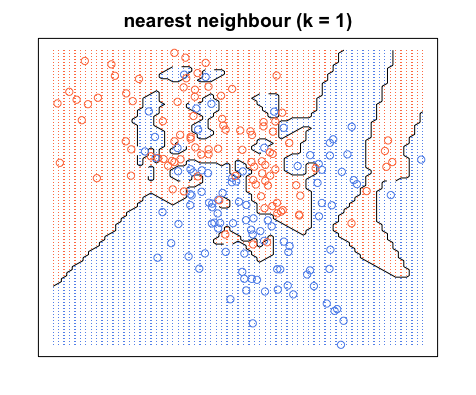
\includegraphics[width=1\linewidth]{figures/03/1nearestneighbor.png}
\caption{ \tiny When k is small, we are restraining the region of a given prediction and forcing our classifier to be “more blind” to the overall distribution. A small value for k provides the most flexible fit, which will have low bias but high variance. Graphically, our decision boundary will be more jagged.}
%link: https://kevinzakka.github.io/2016/07/13/k-nearest-neighbor/
\end{minipage}%
\begin{minipage}{.5\textwidth}
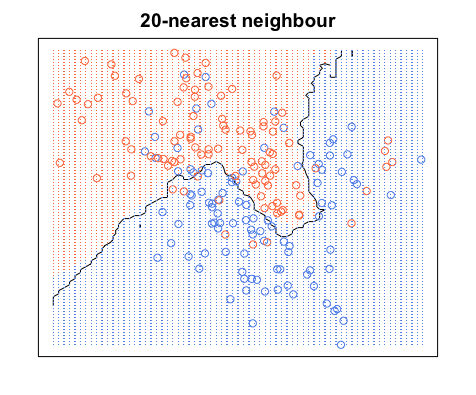
\includegraphics[width=1\linewidth]{figures/03/20nearestneighbor.png}
\caption{ \tiny On the other hand, a higher k averages more voters in each prediction and hence is more resilient to outliers. Larger values of k will have smoother decision boundaries which means lower variance but increased bias}
\end{minipage}
\end{figure}

\end{frame}


\begin{frame}
\frametitle{pros \& cons of k-NN}
\begin{itemize}
\item simple to understand and easy to implement
\item  it can be a useful tool for off-the-bat analysis of some data set you are planning to run more complex algorithms on
\item computationally expensive testing phase which is impractical in industry settings (need to calculate a distance for each data point)
\item Furthermore, KNN can suffer from skewed class distributions. For example, if a certain class is very frequent in the training set, it will tend to dominate the majority voting of the new example (large number = more common)
\end{itemize}
\end{frame}

%------------------------------------------------


%------------------------------------------------



%------------------------------------------------

\begin{frame}
\Huge{\centerline{The End}}
\end{frame}

%----------------------------------------------------------------------------------------

\end{document}